\documentclass[
        a4paper,
        10pt,
        parskip = full,    % Layout with zero \parident and non-zero \parskip
    ]{scrartcl}
% \usepackage[utf8]{inputenc}

\usepackage[top=2cm, bottom=2.5cm, left=2.5cm, right=3cm]{geometry}
\usepackage[
        colorlinks = true,    % Disable drawing boxes around links.
        linkcolor = black,    % Sets the color of links to black.
    ]{hyperref}
\usepackage{amsmath}
\usepackage{graphicx}
\usepackage{subfig}
\usepackage{float}

\begin{document}

\textbf{\large{Laboratory - Deep Learning Lab, WS 2018/2019 - Exercise 1}}

\textbf{\large{Submitted by: Amadeus Hovekamp,\\
amadeus.hovekamp@rwth-aachen.de,\\
Matr. no: 4603934}}

The repository with the source code can be found under the following link:\\
\href{https://github.com/Schokokugel/RoboticsLab}
     {https://github.com/Schokokugel/RoboticsLab}

\section{Activation Functions}
First, let's look at the activation functions. All implemented derivatives seem to be correct.
The gradient check function agrees and shows differences between numerical and analytical derivative smaller than $10^{-7}$, so there are no assertion errors.

\begin{figure}[H]
	\centering
	\subfloat{{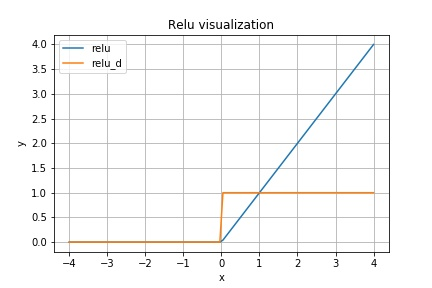
\includegraphics[width=5cm]{../images/activation_functions/relu.jpg} }}
	\subfloat{{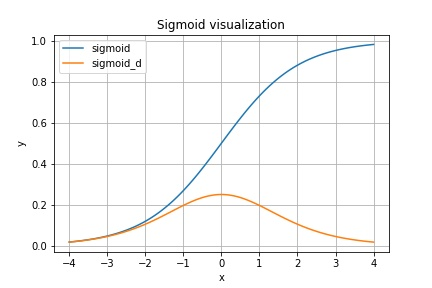
\includegraphics[width=5cm]{../images/activation_functions/sigmoid.jpg} }}	
	\subfloat{{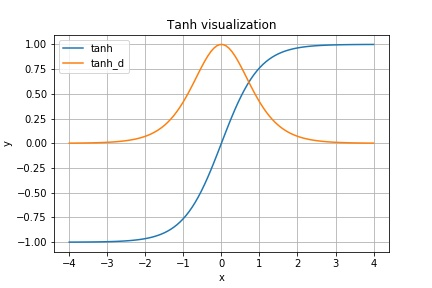
\includegraphics[width=5cm]{../images/activation_functions/tanh.jpg} }}	
    	\caption{ReLU, Sigmoid and Tanh Activation Functions}
\label{fig1}
\end{figure}

\section{Network architectures}

After implementing all ToDos that needed to build the network and the stochastic gradient descent, I trained a relatively small network with 3 hidden layers containing 40 neurons each.
Having heard that ReLU is widely used in neural networks nowadays, I chose to use only ReLU activation functions first.

\begin{figure}[H]
	\centering
	\subfloat{{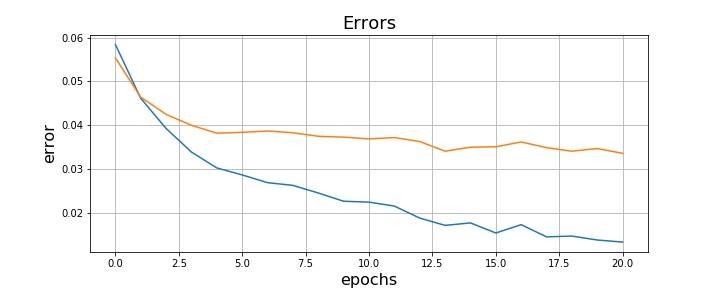
\includegraphics[width=7.5cm]{../images/40_r_40_r_40_r_Errors.jpg} }}
	\subfloat{{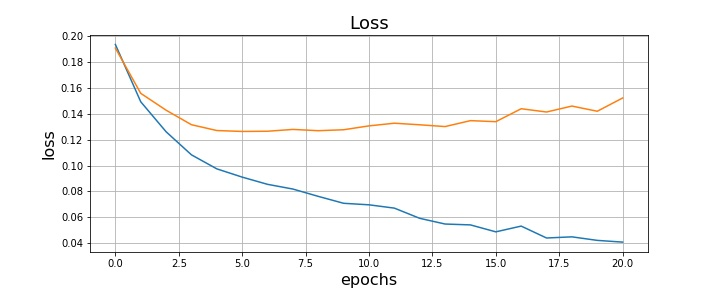
\includegraphics[width=7.5cm]{../images/40_r_40_r_40_r_Losses.jpg} }}	
	\caption{40 ReLU, 40 ReLU, 40 ReLU}
	\label{Small ReLU network}
\end{figure}

It took some time to train this network with all the 50000 training data points but the performance was kind of good already. The training error goes down fast to 1.1 \% and the validation error more slowly to 3.5 \%. But while the training loss goes down to 0.04, the validation loss actually increases after epoch 4 and continues to go up until the end of training. \\

Because it took so long to run the training with all data points, I took a subset of 5000 points to get a feel how the other activation functions perform. While the Tanh activation function was pretty similar to the performance of ReLU, the remaining error of the MLP using the Sigmoid activation function was higher. This may be ok to reduce overfitting but the Sigmoid network did not seem to learn too much even after two rounds training. For this reason I continued playing arround for the most part with ReLUs.

After using both training sets with 5000 and 10000 data points I noticed a big difference in validation error for small networks. The training error went down faster with fewer data points but the validation error remained large. So I realized that 5000 and most probably 10000 are too few data points to get good results.

Due to that I run 3 networks with more neurons over night, (200, 100), (300, 200) and (300, 100, 100). All had kind of good results but stopped improving after about 35 epochs as the training error went down to 0.

\begin{figure}[H]
	\centering
	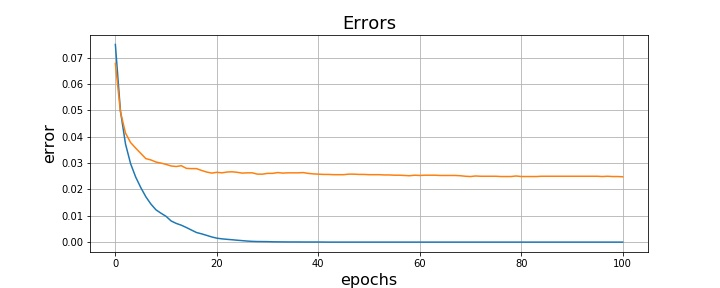
\includegraphics[width=0.7\textwidth]{../images/nn_200r100r_Errors.jpg}
	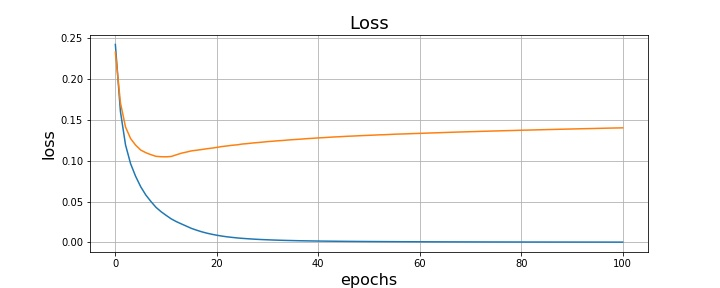
\includegraphics[width=0.7\textwidth]{../images/nn_200r100r_Losses.jpg}	
	\caption{200 ReLU, 100 ReLU}
	\label{nn_200r100r}
\end{figure}
\begin{figure}[H]
	\centering
	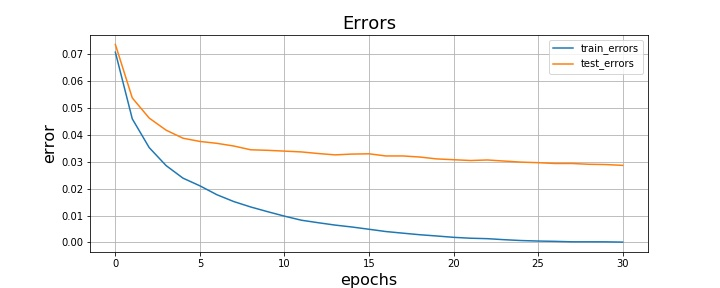
\includegraphics[width=0.7\textwidth]{../images/nn_300r200r_test_Errors.jpg}
	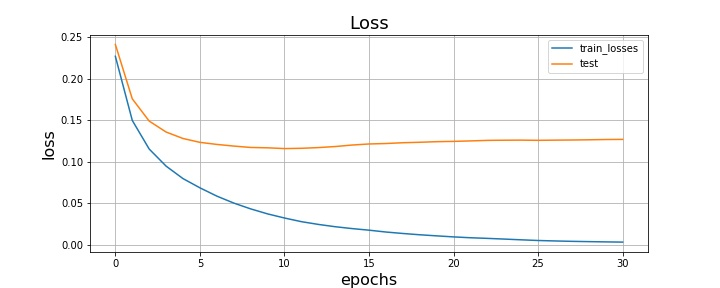
\includegraphics[width=0.7\textwidth]{../images/nn_300r200r_test_Losses.jpg}	
	\caption{300 ReLU, 200 ReLU}
	\label{nn_300r200r}
\end{figure}
\begin{figure}[H]
	\centering
	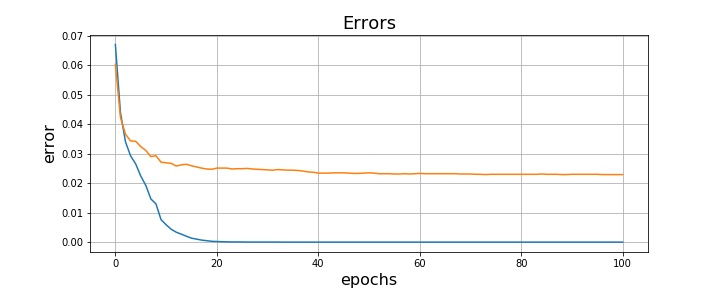
\includegraphics[width=0.7\textwidth]{../images/nn_300r100r100r_Errors.jpg}
	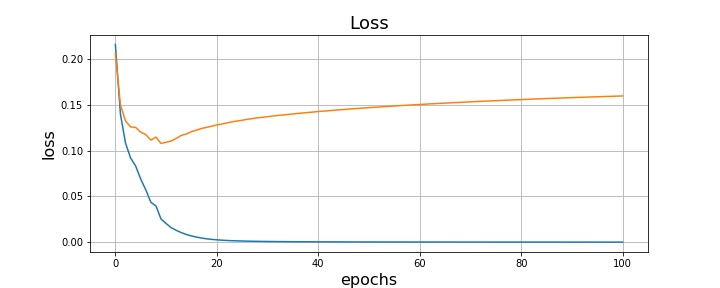
\includegraphics[width=0.7\textwidth]{../images/nn_300r100r100r_Losses.jpg}	
	\caption{300 ReLU, 100 ReLU, 100 ReLU}
	\label{nn_300r100r100r}
\end{figure}

\section{Gradient Descent vs. SGD}

As Gradient Descent performed way worse than SGD I stopped using it after several runs with different architectures.

\section{Evaluation}

I trained (300, 200) with ReLUs with 0.08 learning rate, batch size 80 and 30 epochs. It achieved a final test error of 0.0287 which is worse than I expected. 


\end{document}
